
\documentclass[conference]{IEEEtran}
\usepackage{graphicx}
\usepackage{float}
\usepackage{url}

\title{Automated measurement of fetal head circumference using 2D ultrasound images}

\author{
\IEEEauthorblockN{Nguyen Tuan Thanh}
\IEEEauthorblockA{
Student ID: 22BA13289 \\
University of Science and Technology of Ha Noi (USTH) \\
Email: thanhnt.22ba13289@usth.edu.vn
}
}

\begin{document}

\maketitle

\section{Exploratory Data Analysis}
\subsection{Dataset Overview}


\subsubsection{Training Set}

The training set is provided in the file training\_set\_pixel\_size\_and\_HC.csv. It contains 999 ultrasound images. Each image is associated with the following attributes:

\begin{itemize}
    \item \textbf{filename}: the name of the ultrasound image file.
    \item \textbf{pixel size (mm)}: the physical size of one pixel in millimeters, depending on the ultrasound machine settings.
    \item \textbf{head circumference (mm)}: the ground-truth HC value obtained from manual annotation by fitting an ellipse to the fetal head boundary.
\end{itemize}

\subsubsection{Test Set}
The test set is provided in the file test\_set\_pixel\_size.csv. It contains 335 ultrasound images. Each sample includes:

\begin{itemize}
    \item \textbf{filename}: the name of the ultrasound image file.
    \item \textbf{pixel size (mm)}: the physical size of one pixel in millimeters.
\end{itemize}

The test set does not include ground-truth HC values. These are predicted by the trained model.

\subsection{Class Distribution}

\begin{figure}[H]
    \centering
    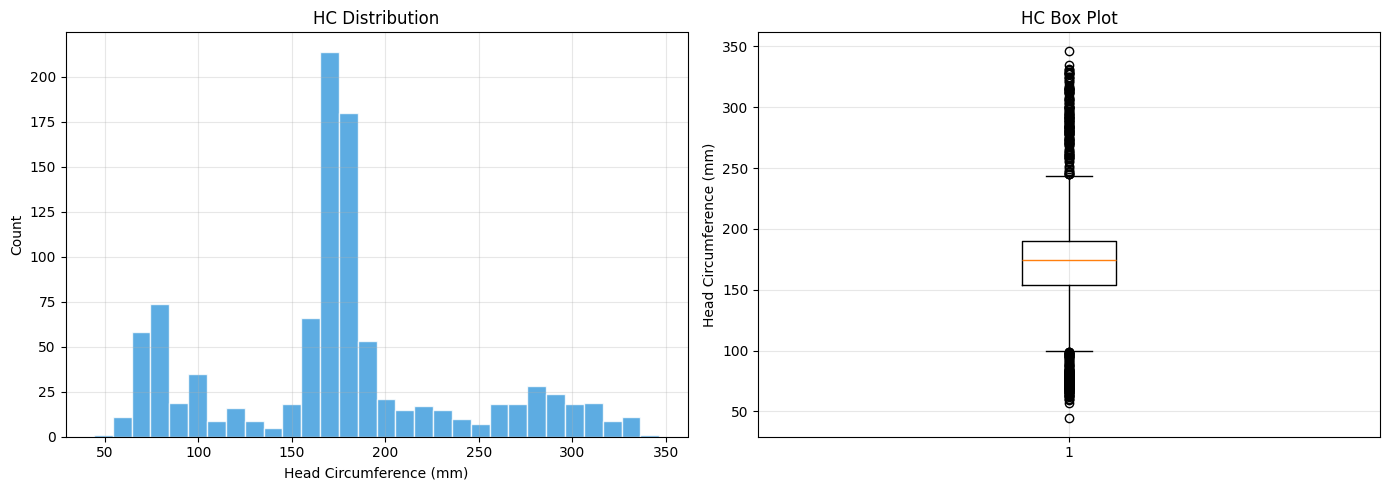
\includegraphics[width=0.9\linewidth]{figures/figure_1.png}
    \caption{Distribution of head circumference in the training set (histogram and box plot)}
    \label{fig:train_hc}
\end{figure}

The HC values in the training set range from approximately 44\,mm to 346\,mm, with a mean of 174.38\,mm and a standard deviation of 65.28\,mm. The histogram shows that the distribution has a prominent peak around 170--190\,mm, with additional smaller peaks at lower HC values (around 60--80\,mm). This suggests the dataset includes fetuses from early to late gestational ages. The box plot confirms a wide interquartile range (153.6--189.8\,mm) with several outliers at both extremes, indicating high variability in the data.

\begin{figure}[H]
    \centering
    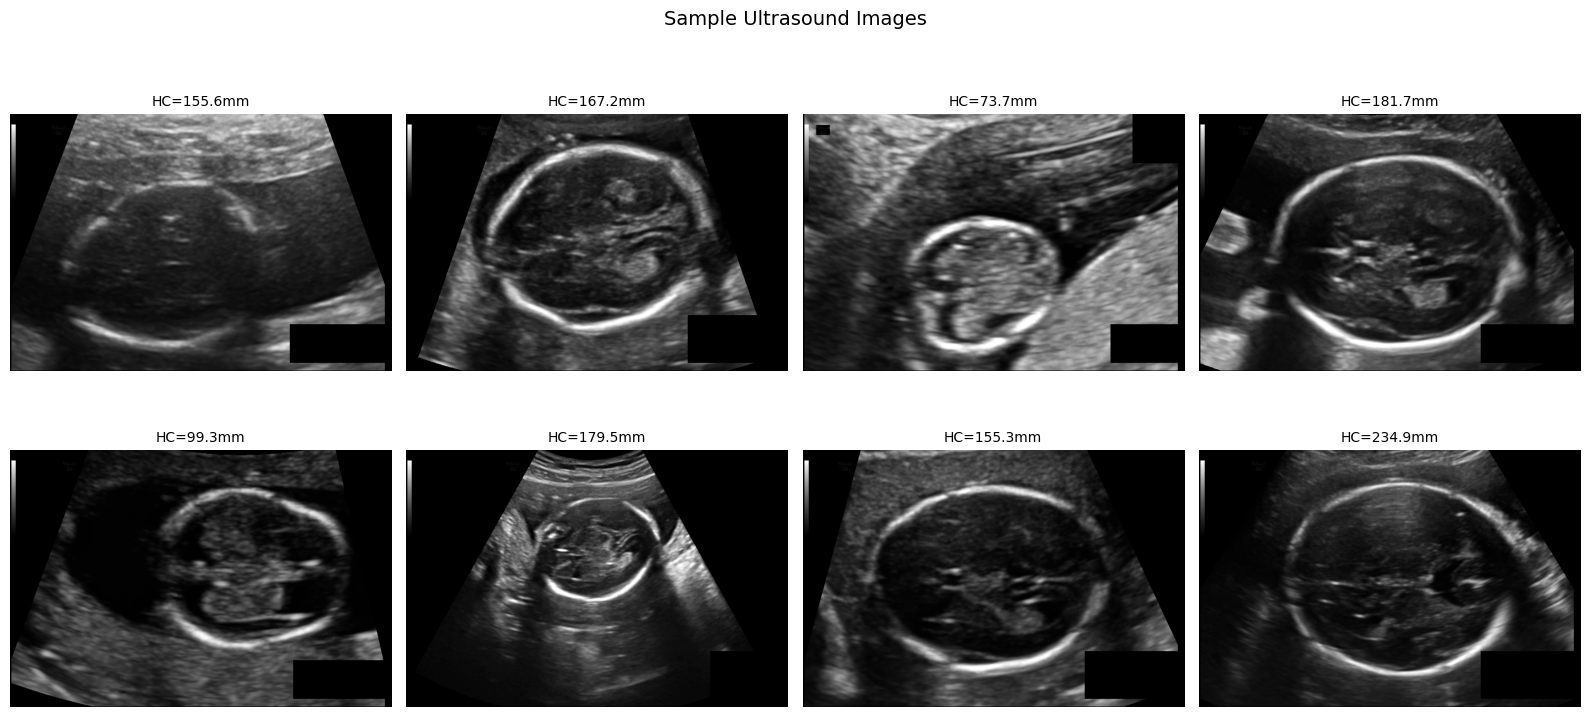
\includegraphics[width=0.9\linewidth]{figures/figure_2.png}
    \caption{Sample ultrasound images from the training set with their HC values}
    \label{fig:sample_images}
\end{figure}

Sample images from the training set show substantial variation in image quality, contrast, and the orientation and size of the fetal head. Some images display clear, well-defined head boundaries, while others have lower contrast or contain imaging artifacts. The HC values shown above each image range from 73.7\,mm to 234.9\,mm, reflecting the diversity in fetal development stages present in the dataset.

\subsection{Conclusion and Insights from EDA}

From the exploratory data analysis:

\begin{itemize}
    \item The HC values cover a wide range from very small to very large measurements (44.3--346.4\,mm). This indicates the dataset spans many gestational ages and makes the regression task challenging, as the model must handle large variations in both image appearance and target values.
    \item The dataset contains 999 training images, which is relatively small for deep learning. Transfer learning from a pre-trained model is therefore essential to achieve reasonable performance.
    \item Sample images show significant diversity in terms of image quality, fetal position, and head size. A model with strong feature extraction capabilities is needed to capture the relevant visual patterns.
\end{itemize}

Overall, the dataset is realistic and diverse. It is suitable for training and evaluating a regression model for fetal HC estimation.



\subsection{Model Implementation}

\subsubsection{Data Loading}

Two CSV files are used in this work:
\begin{itemize}
    \item The training file contains image filenames and ground-truth HC values.
    \item The test file contains image filenames only.
\end{itemize}

Two image folders are defined: \texttt{training\_set/} and \texttt{test\_set/}. The filename column and the HC column are automatically detected from the CSV headers using keyword matching to make the code robust to minor column name variations.

\subsubsection{Image Preprocessing}

Each ultrasound image is processed as follows:
\begin{itemize}
    \item The image is loaded in grayscale.
    \item The image is resized to $224 \times 224$ pixels.
    \item Pixel values are normalized to the range $[0,1]$.
    \item The data are reshaped to $(N, 224, 224, 1)$.
\end{itemize}

If a filename does not match an existing file, multiple filename formats and extensions are checked. Samples with missing images or invalid HC values are removed from the dataset.

\subsubsection{Train--Validation Split}

The training set is split into training and validation subsets using an 80/20 ratio. A fixed random seed is used to ensure reproducible results.

\subsubsection{Network Architecture}

An EfficientNetB0 model pre-trained on ImageNet is used as the backbone feature extractor. The classification head is removed by setting \texttt{include\_top=False}. The input shape of the backbone is $(224, 224, 3)$.

Since the input images are single-channel grayscale, they are first converted to 3-channel RGB using a \texttt{Lambda} layer with \texttt{grayscale\_to\_rgb}. The EfficientNet preprocessing function is then applied to rescale pixel values.

The regression head consists of:
\begin{itemize}
    \item A Global Average Pooling layer.
    \item A fully connected layer with 128 units and ReLU activation.
    \item A Batch Normalization layer.
    \item A Dropout layer with rate 0.3.
    \item A fully connected layer with 64 units and ReLU activation.
    \item A Dropout layer with rate 0.2.
    \item A final fully connected layer with one output for regression.
\end{itemize}

During training, the backbone network is frozen and only the regression head is updated. The model has 4,222,372 total parameters, of which 172,545 are trainable.

\subsubsection{Training Setup}

The model is trained with the following settings:
\begin{itemize}
    \item Optimizer: Adam with learning rate $5 \times 10^{-4}$.
    \item Loss function: Mean Absolute Error (MAE).
    \item Batch size: 16.
    \item Maximum number of epochs: 30.
\end{itemize}

Two callbacks are used:
\begin{itemize}
    \item Early Stopping on validation MAE with patience 7 and best weight restoration.
    \item ReduceLROnPlateau on validation MAE with factor 0.5, patience 3, and minimum learning rate $10^{-6}$.
\end{itemize}

The model weights with the best validation MAE are restored at the end of training.

\subsubsection{Evaluation}

After training, the model is evaluated on the validation set. The following regression metrics are reported:
\begin{itemize}
    \item Mean Absolute Error (MAE),
    \item Root Mean Squared Error (RMSE),
    \item Coefficient of determination ($R^2$).
\end{itemize}

These metrics provide a clear view of the prediction error and the overall goodness of fit.

\subsubsection{Test Prediction and Submission}

For the test set, the same preprocessing steps are applied. The trained model is used to generate predictions, which are saved to a CSV file containing two columns:
\begin{itemize}
    \item filename,
    \item HC.
\end{itemize}

This file is used as the final submission.


\section{Experimental Results}

In this section, we present the experimental results of the EfficientNetB0-based model for fetal head circumference estimation. The performance is evaluated on the validation set using standard regression metrics.

\subsection{Evaluation Metrics}

To evaluate the regression performance, we use three common metrics:

\begin{itemize}
    \item Mean Absolute Error (MAE)
    \item Root Mean Squared Error (RMSE)
    \item Coefficient of Determination ($R^2$)
\end{itemize}

\subsection{Training Process}

The model is trained for 30 epochs on the training subset and evaluated on the validation set at each epoch.

\begin{figure}[H]
    \centering
    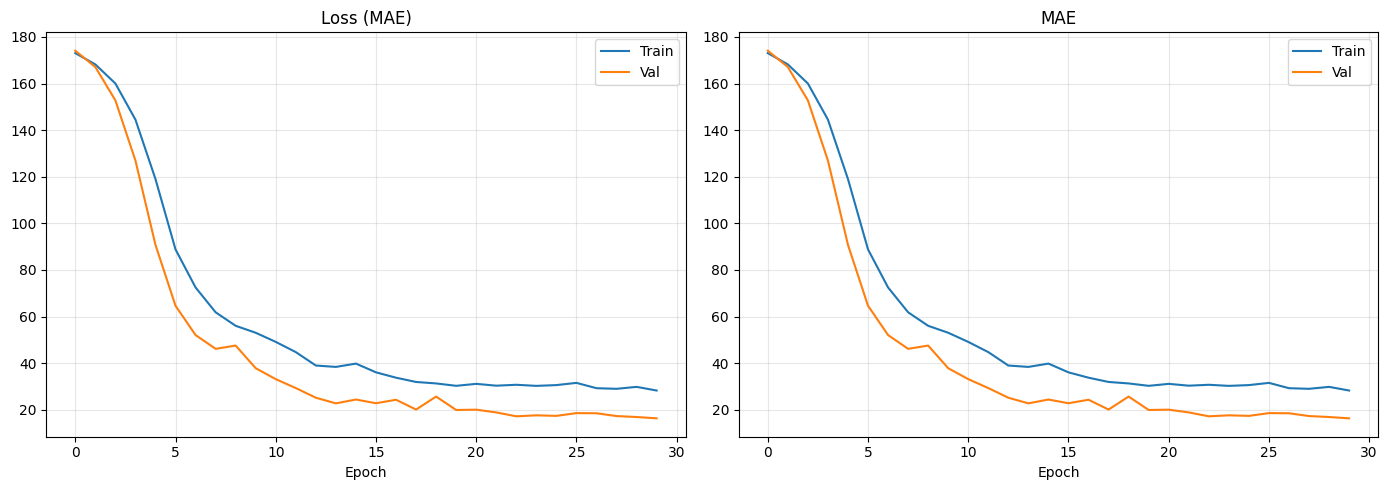
\includegraphics[width=0.9\linewidth]{figures/figure_4.png}
    \caption{Training and validation loss (MAE) over epochs}
    \label{fig:training_history}
\end{figure}

Figure~\ref{fig:training_history} shows the training and validation MAE curves over 30 epochs. Both curves decrease rapidly in the first 10 epochs and then converge more slowly. The ReduceLROnPlateau callback reduced the learning rate from $5 \times 10^{-4}$ to $2.5 \times 10^{-4}$ around epoch 18, and further to $1.25 \times 10^{-4}$ around epoch 27. Early Stopping did not trigger, indicating continued improvement throughout all epochs.

A notable observation is that the validation MAE is consistently lower than the training MAE after the first few epochs. This is due to Dropout being active during training but inactive during validation, as well as Batch Normalization computing running statistics differently between training and inference modes.

\subsection{Quantitative Results}

Table~\ref{tab:results} shows the regression performance of the model on the validation set.

\begin{table}[H]
\centering
\caption{Performance on the validation set}
\label{tab:results}
\begin{tabular}{lccc}
\hline
Metric & MAE (mm) & RMSE (mm) & $R^2$ \\
\hline
EfficientNetB0-based model & 16.34 & 21.82 & 0.8863 \\
\hline
\end{tabular}
\end{table}

The results show that the model can predict the head circumference with a reasonable error. The $R^2$ score of 0.8863 indicates that the model explains approximately 89\% of the variance in the data. The MAE of 16.34\,mm corresponds to roughly 5.4\% relative error over the full HC range (44.3--346.4\,mm).

\begin{figure}[H]
    \centering
    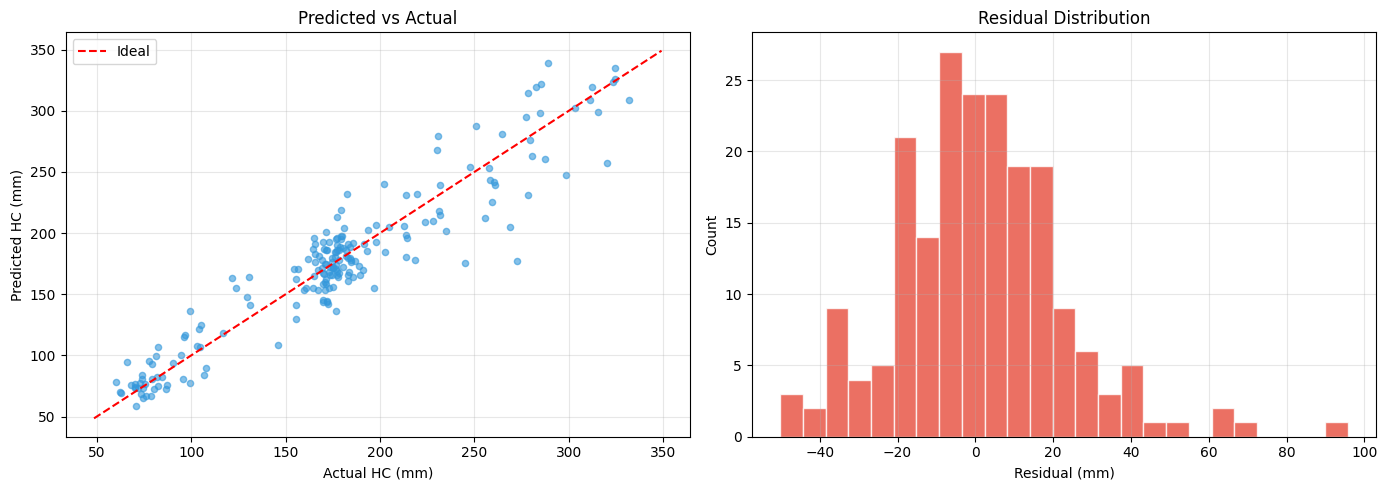
\includegraphics[width=0.9\linewidth]{figures/figure_3.png}
    \caption{Predicted vs.\ actual HC values (left) and residual distribution (right)}
    \label{fig:pred_vs_actual}
\end{figure}

Figure~\ref{fig:pred_vs_actual} provides a visual assessment of the model's predictions. The scatter plot (left) shows that most predictions follow the ideal diagonal line, with some scatter increasing for larger HC values. The residual distribution (right) is approximately centered around zero, indicating no systematic bias, though some residuals extend to $\pm$50\,mm for difficult cases.

\subsection{Discussion}

Overall, the experimental results demonstrate that the EfficientNetB0-based regression model is able to learn useful features from ultrasound images and estimate fetal head circumference with reasonable accuracy. However, there is still room for improvement, especially for samples with extreme HC values.


\section{Comparison with HC18 Leaderboard}
Results on the validation set are compared with representative methods from the HC18 Grand Challenge leaderboard. Methods on this leaderboard typically use segmentation followed by ellipse fitting to derive head circumference.

\subsection{Comparison with Published Results}

State-of-the-art methods from the HC18 leaderboard achieve mean absolute differences below 2\,mm through segmentation-based approaches. These methods typically use U-Net or similar architectures to segment the fetal head boundary at the pixel level, then compute the circumference from the fitted ellipse.

While direct comparison across different evaluation protocols is not fully standardized, the large difference in error magnitude indicates that segmentation-based pipelines currently outperform simple regression approaches in terms of absolute accuracy.

\subsection{Discussion}

The comparison highlights a clear trade-off in fetal head circumference estimation. Segmentation-based methods achieve higher accuracy but require detailed pixel-level annotations and complex multi-stage pipelines, while the proposed regression-based approach provides a simpler and annotation-efficient alternative at the cost of higher error.

\section{Conclusion}

In this work, we studied the problem of estimating fetal head circumference from 2D ultrasound images using a deep learning approach. Instead of a traditional segmentation-based pipeline, we proposed a regression-based method that directly predicts the HC value from the input image using an EfficientNetB0-based network with a frozen pre-trained backbone.

Experimental results show that the model learns meaningful visual features and achieves an $R^2$ of 0.8863 on the validation set, with an MAE of 16.34\,mm and RMSE of 21.82\,mm. Although the error is significantly higher than state-of-the-art segmentation-based methods on the HC18 benchmark, the proposed approach provides a much simpler pipeline and does not require pixel-level annotations.

This demonstrates a clear trade-off between accuracy and complexity: segmentation-based methods produce more precise measurements but need detailed annotations and multi-stage processing, while the regression approach is lightweight and annotation-efficient.

In future work, performance can be improved by fine-tuning the backbone on ultrasound data, applying data augmentation, using a stronger backbone, or employing multi-task learning.


\begin{thebibliography}{2}

\bibitem{hc18}
T. L. A. van den Heuvel et al.,
``Automated measurement of fetal head circumference using 2D ultrasound images,''
\textit{PLoS ONE}, vol. 13, no. 8, 2018.
[Online]. Available: \url{https://hc18.grand-challenge.org/}

\bibitem{efficientnet}
M. Tan and Q. V. Le,
``EfficientNet: Rethinking Model Scaling for Convolutional Neural Networks,''
\textit{Proc. Int. Conf. Machine Learning (ICML)}, 2019.

\end{thebibliography}


\end{document}
